%\chapter*{Неделя 10}
\protect\thispagestyle{fancy}
\section{}
Передаточная функция цифрового фильтра имеет вид

\begin{equation*}
	\Capit{H}(z) = \dfrac{1 - 2z^{-1} + z^{-2}}{1 - \frac{1}{2}z^{-1} - \frac{1}{2}z^{-2}}.
\end{equation*}

Изобразить блок-схемы цифрового фильтра в прямой и канонической формах и записать соответствующие разностные уравнения (алгоритмы цифровой фильтрации).

\begin{align*}
	&\Capit{H}(z)\footnotemark = \dfrac{1 - 2z^{-1} + z^{-2}}{1 - \frac{1}{2}z^{-1} - \frac{1}{2}z^{-2}} = \dfrac{\Capit{Y}(z)}{\Capit{X}(z)}.\\
	\Capit{Y}(z)\Big(1 - \frac{1}{2}z^{-1} - \frac{1}{2}z^{-2}\Big) =
	\Capit{X}(z)\Big(1 &- 2z^{-1} + z^{-2}\Big) \xlongleftrightarrow{\Capit{Z}} 
	y[k] - \dfrac{1}{2}y[k-1] - \dfrac{1}{2}y[k-2] = x[k] - 2x[k-1] + x[k-2].\\
	y[k] = x[k]& - 2x[k-1] + x[k-2] + \dfrac{1}{2}y[k-1] + \dfrac{1}{2}y[k-2].
\end{align*}

\begin{figure}[!h]
	\centering
	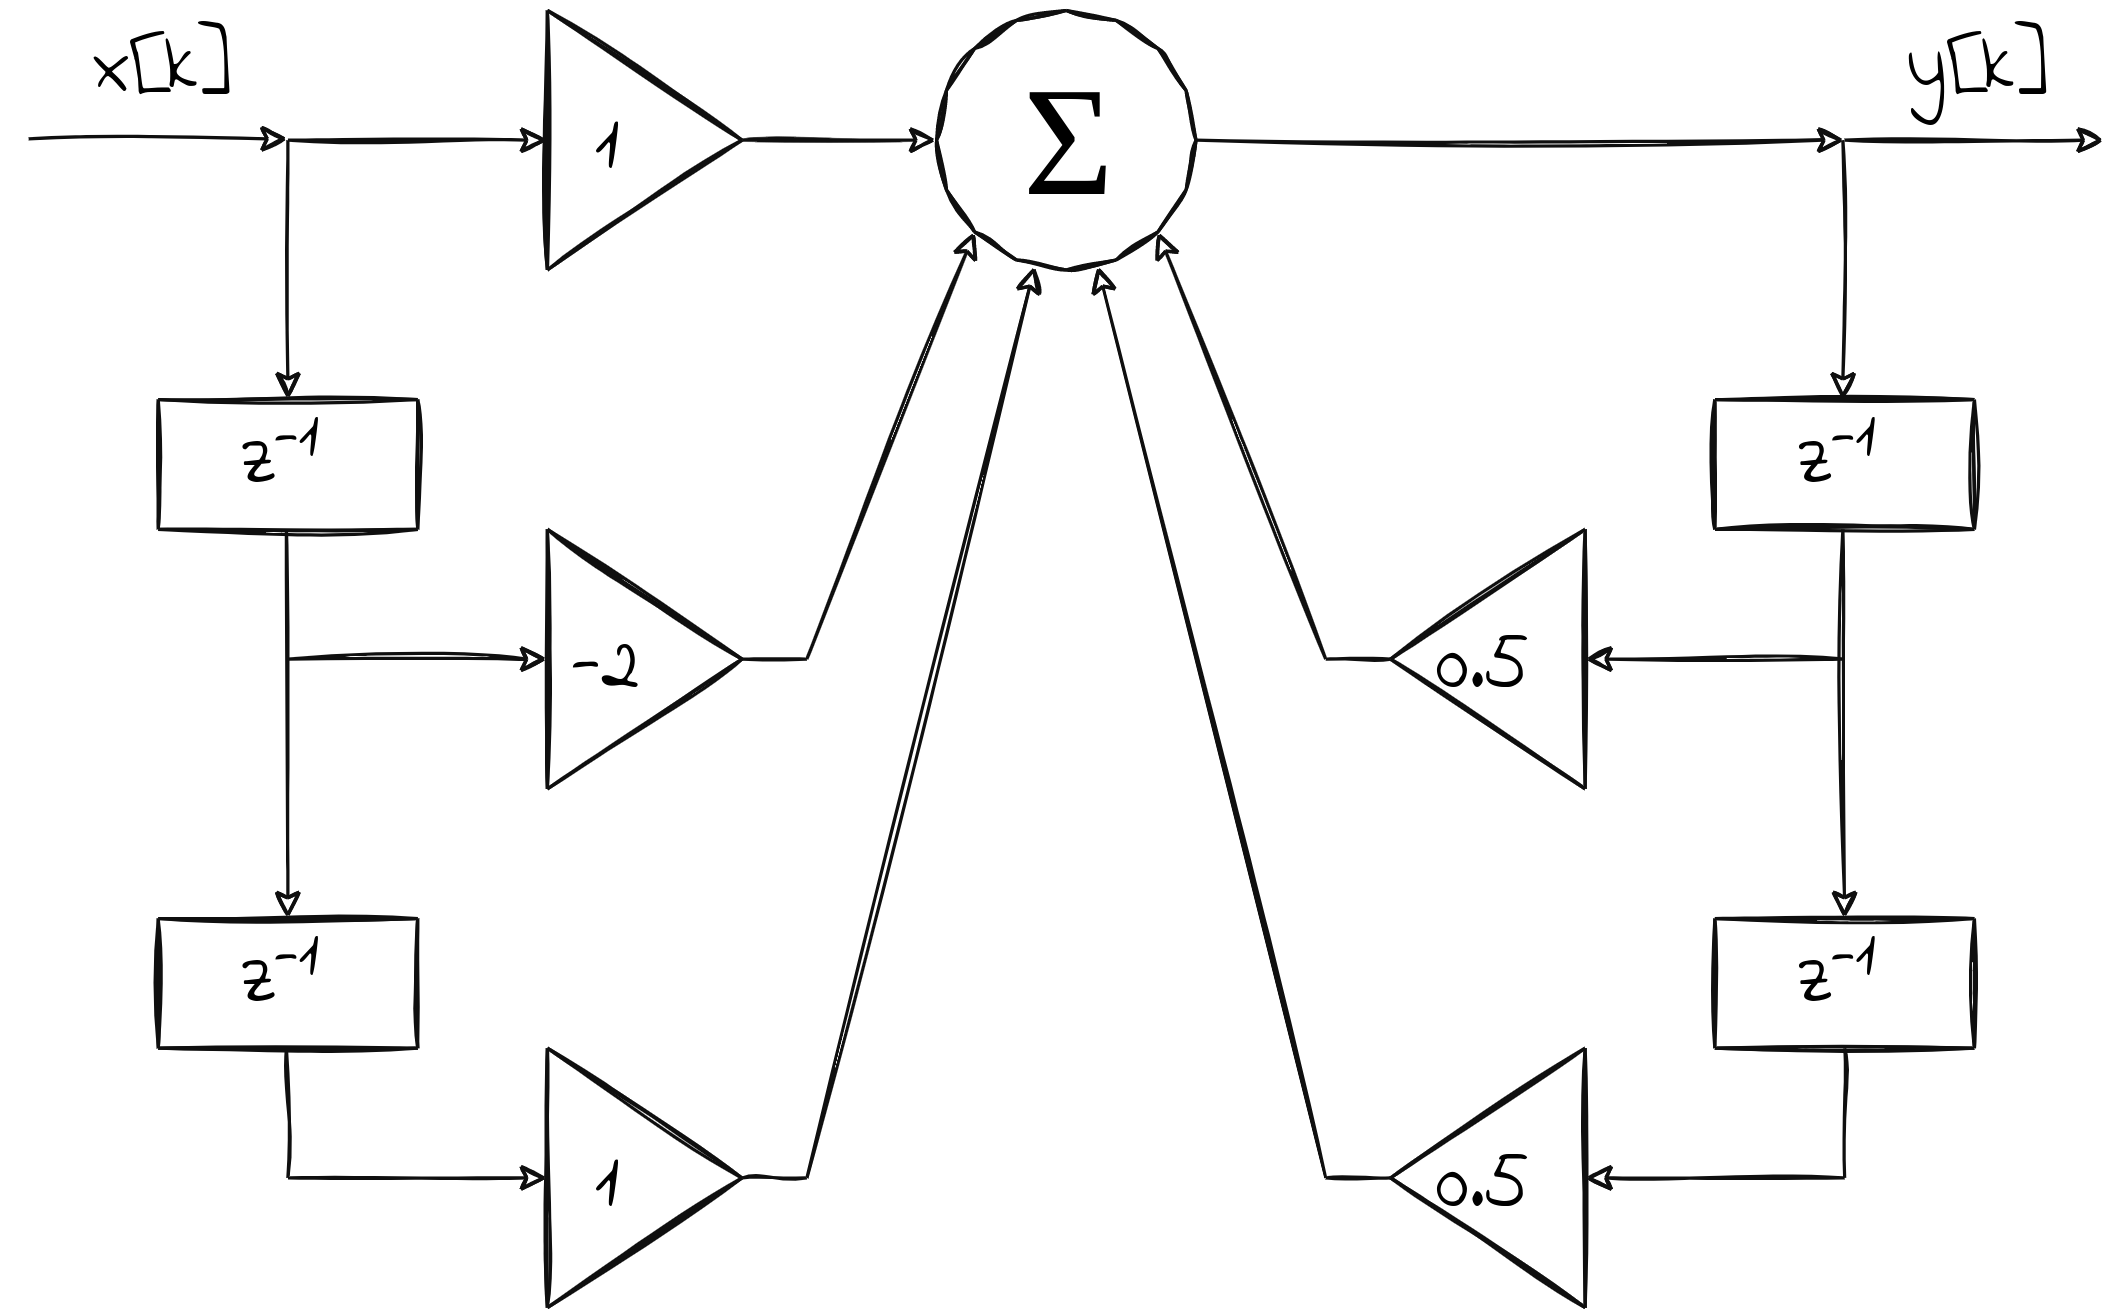
\includegraphics[width=0.6\columnwidth]{pics/fall/10/10-1.png}
	\caption{Прямая форма фильтра.}
	\label{fig:10-1}
\end{figure}

\begin{figure}[!h]
	\centering
	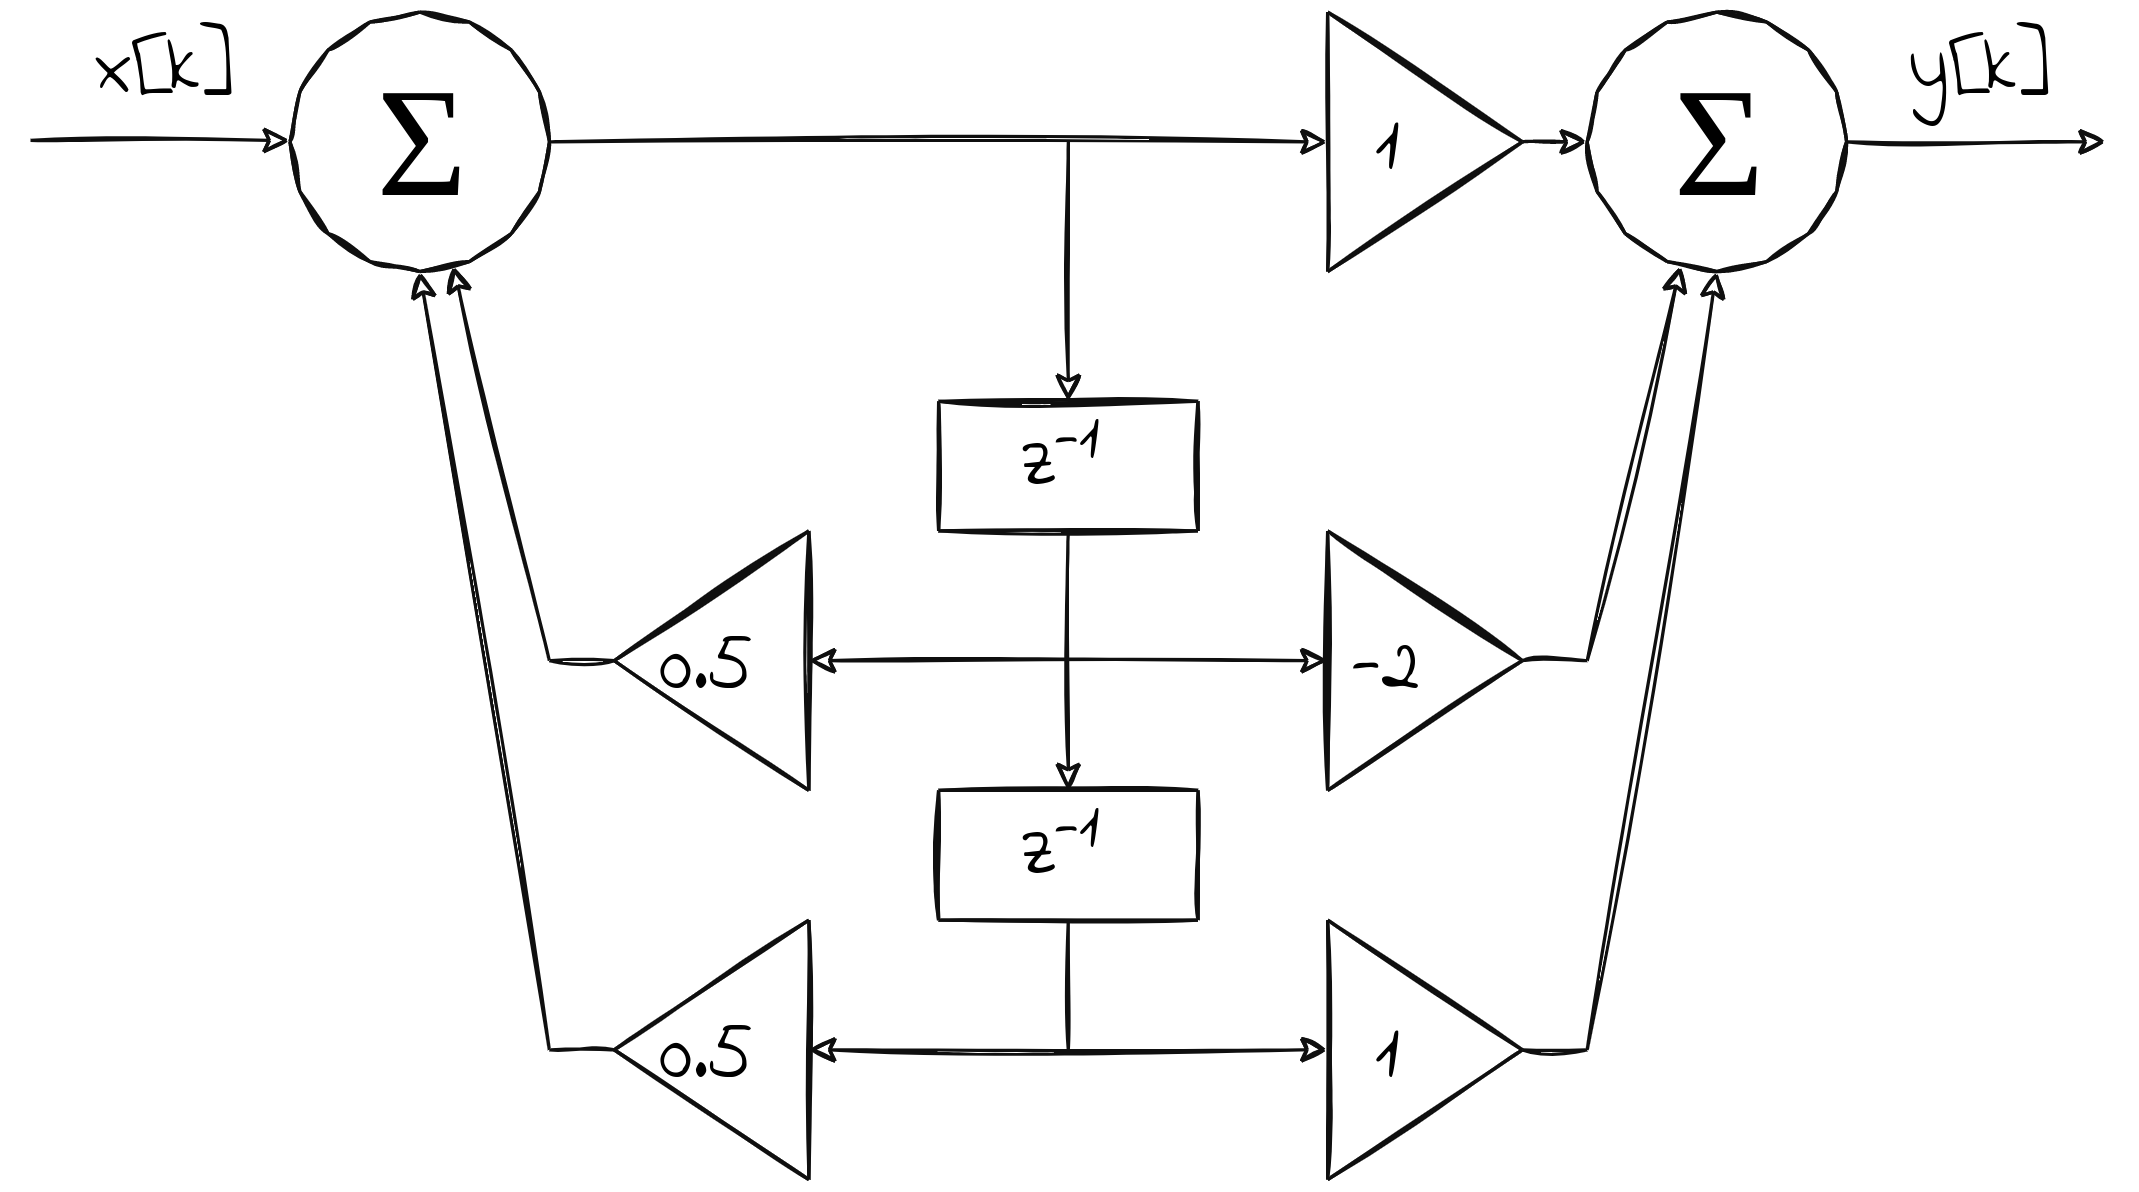
\includegraphics[width=0.6\columnwidth]{pics/fall/10/10-2.png}
	\caption{Каноническая (прямая) форма фильтра.}
	\label{fig:10-2}
\end{figure}

\footnotetext{В данном случае $\Capit{H}(z)$ содержит компенсирующие друг друга нуль и полюс. Иными словами, передаточная функция допускает упрощение. Однако схемы реализации построены для исходного вида $\Capit{H}(z)$, так как после сокращения формально получится другая передаточная функция.}

\newpage 
\section{}
Изобразить блок-схему одной из возможных реализаций фильтра с передаточной функцией

\begin{equation*}
	\Capit{H}(z) = \dfrac{0.5477 + 0.9322z^{-1} + 0.5466z^{-2}}
	{1 - 0.6106z^{-1} + 0.3029z^{-2}} \cdot
	\dfrac{0.1906 + 0.1689z^{-1} + 0.1906z^{-2}}
	{1 - 0.0013z^{-1} + 0.8093z^{-2}}
\end{equation*}

в виде каскада двух биквадратных блоков. Для биквадратных блоков выбрать прямую каноническую форму реализации.

\begin{figure}[!h]
	\centering
	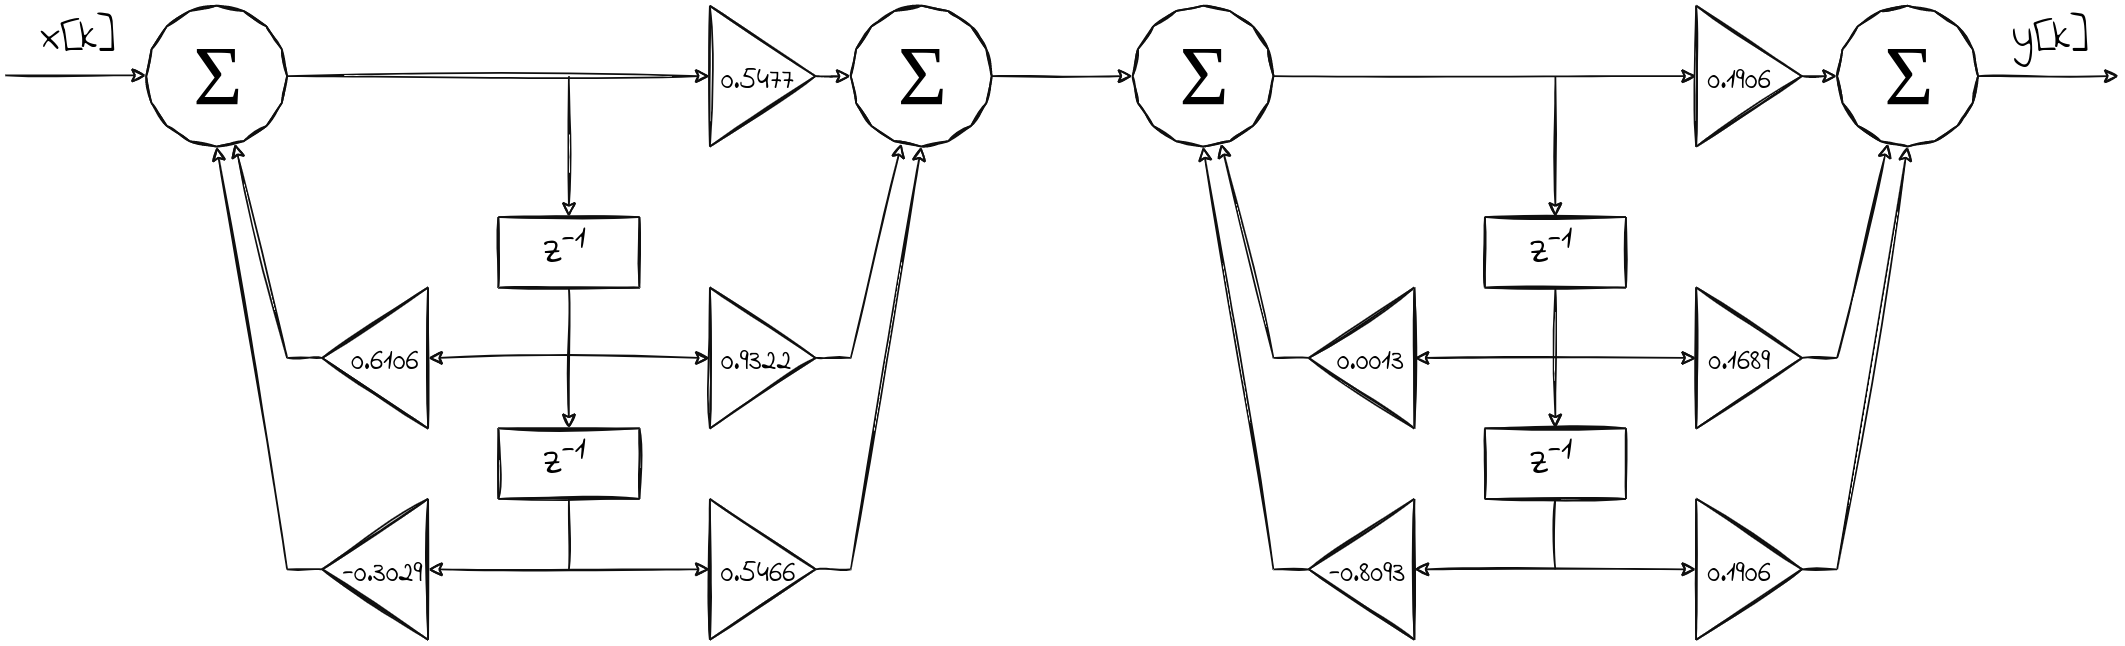
\includegraphics[width=1.0\columnwidth]{pics/fall/10/10-3.png}
	%\caption{Каноническая (прямая) форма фильтра.}
	\label{fig:10-3}
\end{figure}


\section{}
Изобразить в прямой форме блок-схему реализации цифрового фильтра второго порядка, у передаточной функции которого два комплексно-сопряжённых нуля $z_{1, 2} = \pm 0.5j$ и два комплексно-сопряжённых полюса $z_{3,4} = \pm 0.2j$, а значение частотной характеристики на частоте $0$ равно $1.28$.

\begin{align*}
	&\Capit{H}(z) = \s{k}\dfrac{(z - z_1)(z - z_2)}{(z - z_3)(z - z_4)} = \s{k}\dfrac{(z - z_1)(z - z_1^*)}{(z - z_3)(z - z_3^*)} = \s{k} \dfrac{z^2 + |z_1|^2}{z^2 + |z_3|^2} = \s{k}\dfrac{1 + |z_1|^2z^{-2}}{1 + |z_3|^2z^{-2}} = \s{k}\dfrac{1 + 0.25\cdot z^{-2}}{1 + 0.04\cdot z^{-2}}.\\
	&\Capit{H}(z)\big|_{\nu = 0} = \Capit{H}(z)\big|_{z = 1} = \s{k} \dfrac{1 + 0.25}{1 + 0.04} =
	\s{k} \cdot 1.2019 = 1.28,\quad \Rightarrow \s{k} = 1.0650.
\end{align*}

\begin{equation*}
	\Capit{H}(z) =  1.0650 \cdot \dfrac{1 + 0.25\cdot z^{-2}}{1 + 0.04\cdot z^{-2}}.
\end{equation*}

\begin{figure}[!h]
	\centering
	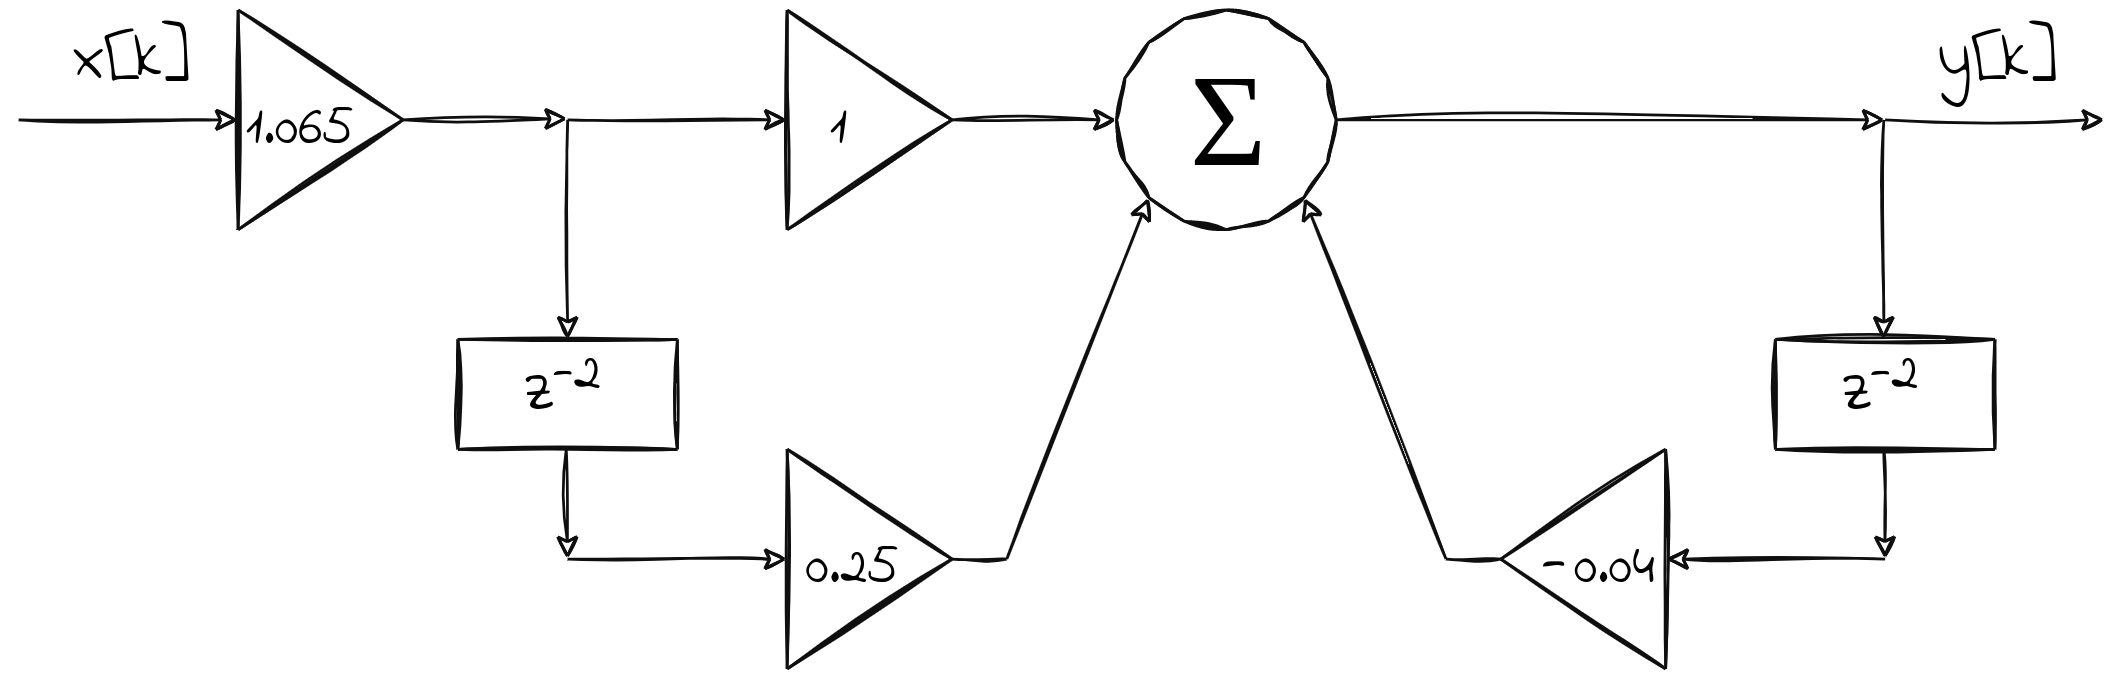
\includegraphics[width=1.0\columnwidth]{pics/fall/10/10-4.png}
	\label{fig:10-4}
\end{figure}

\section{}
Описать переход от прямой формы реализации биквадратного блока к форме, представленной ниже.

\begin{figure}[!h]
	\centering
	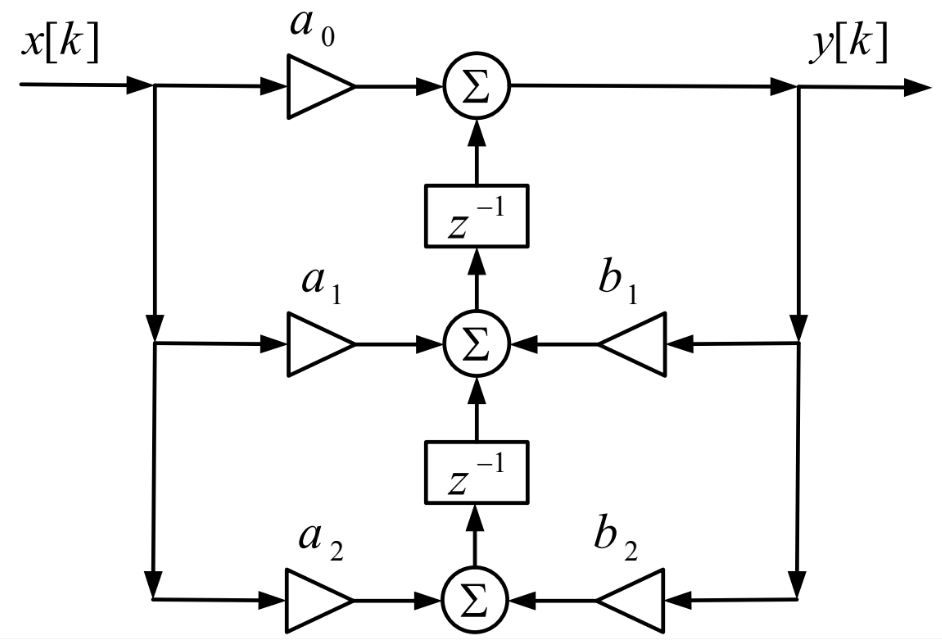
\includegraphics[width=0.6\columnwidth]{pics/fall/10/10-5.png}
	\label{fig:10-5}
\end{figure}

Чтобы получить представленную форму реализации биквадратного блока, необходимо:

\begin{itemize}
	\item поменять в прямой форме реализации последовательность вычисления операций умножения и задержки, используя в каждой ветви отдельную линию задержки на нужное количество тактов; 
	\item разделить общий единый сумматор на несколько двухвходовых сумматоров;
	\item при этом, рассмотрев любую пару соседних сумматоров, можно заметить, что
	суммируемые ими сигналы претерпевают некоторую общую задержку. Это дает возможность поменять местами операции суммирования и задержки.
	
\end{itemize}

